\begin{exercise}{Cascade de Yelowstone}{2}{Sup}
{Optique,Optique géométrique}{lelay,bermudez}

\begin{figure}[H]
    \centering
    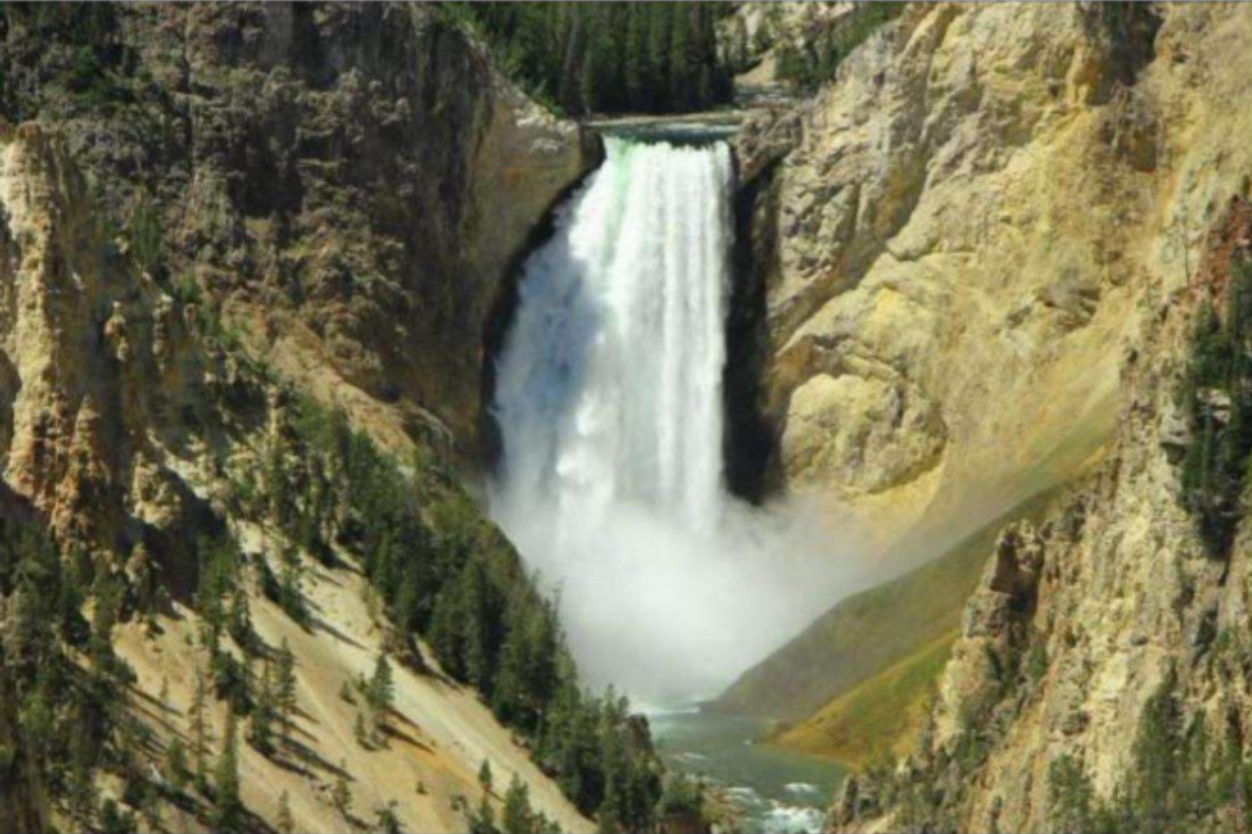
\includegraphics[width=1.\linewidth]{optique/optiquegeometrique/cascade1.png}
    \caption{Photographie de la cascade inférieure de Yellowstone vue de Red Rock Point. \newline (Nikon F, pellicule Kodak Kodachrome 35 format $24\times 36$ mm, téléobjectif $f'= 90$ mm).}
\end{figure}

\begin{figure}[H]
    \centering
    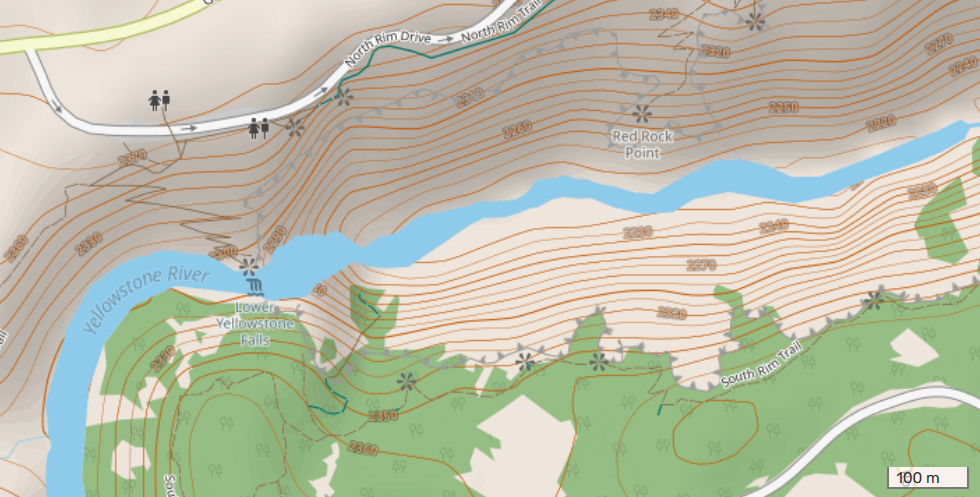
\includegraphics[width=1.\linewidth]{optique/optiquegeometrique/cascade2.png}
    \caption{Carte topographique du Canyon de Yellowstone, avec la cascade inférieure et Red Rock Point.}
\end{figure}

\textsfbf{Problème ouvert :} À l’aide des documents et de vos connaissances, estimer la hauteur de la cascade inférieure de la rivière Yellowstone dans le Grand Canyon (Wyoming, États-Unis). \newline
Valider cet ordre de grandeur en vous aidant des lignes de niveau sur la carte topographique.

\end{exercise}

\begin{solution}
    Relation de conjugaison sur le grandissement :
    $$\gamma = \dfrac{\bar{A'B'}}{\bar{AB}} = -\frac{f'}{\bar{FA}}.$$
    On obtient avec les documents :
    \begin{itemize}
        \item $\bar{A'B'} = -17$ mm
        \item $\bar{FA} \simeq D = \text{distance photographe--cascade} = 245$ m.
        \item $f' = 90$ mm
    \end{itemize}
    D'où $H = \bar{AB} = D\dfrac{-\bar{A'B'}}{f'} = 94$ m.

    On compte bien environ 9 lignes de niveau entre le haut et le bas de la cascade.
\end{solution}